\documentclass[final]{beamer} % beamer 3.10: do NOT use option hyperref={pdfpagelabels=false} !
%\documentclass[final,hyperref={pdfpagelabels=false}]{beamer} % beamer 3.07: get rid of beamer warnings
\mode<presentation> {  %% check http://www-i6.informatik.rwth-aachen.de/~dreuw/latexbeamerposter.php for examples
  \usetheme{qcv}    %% you should define your own theme e.g. for big headlines using your own logos 
}
\usepackage[english]{babel}
\usepackage[latin1]{inputenc}
\usepackage{amsmath,amsthm, amssymb, latexsym}
%\usepackage{times}\usefonttheme{professionalfonts}  % times is obsolete
\usefonttheme[onlymath]{serif}
\boldmath
\usepackage[orientation=landscape,size=a0,scale=1.4,debug]{beamerposter}                       % e.g. for DIN-A0 poster
%\usepackage[orientation=portrait,size=a1,scale=1.4,grid,debug]{beamerposter}                  % e.g. for DIN-A1 poster, with optional grid and debug output
%\usepackage[size=custom,width=200,height=120,scale=2,debug]{beamerposter}                     % e.g. for custom size poster
%\usepackage[orientation=portrait,size=a0,scale=1.0,printer=rwth-glossy-uv.df]{beamerposter}   % e.g. for DIN-A0 poster with rwth-glossy-uv printer check

\title[QCViewer]{QCViewer}
\author[Author]{Author and Author}
\institute[IQC, University of Waterloo]{Quantum Circuits group, IQC, University of Waterloo}
\date{\today}


\begin{document}
  \begin{frame}{} 
  \begin{columns}
   
   % Overview Section
    \begin{column}{.33\textwidth}
      \begin{beamercolorbox}[center,wd=\textwidth]{postercolumn}
         \begin{minipage}[T]{.95\textwidth}
           \begin{block}{\large Overview}
	QCViewer is a tool for displaying, editing, and simulating quantum circuits. It allows users to test new circuit designs and make publication quality diagrams with an easy-to-use graphical interface. Supported features also include simulation of the circuit while graphically displaying the current state. 

             \centering 
             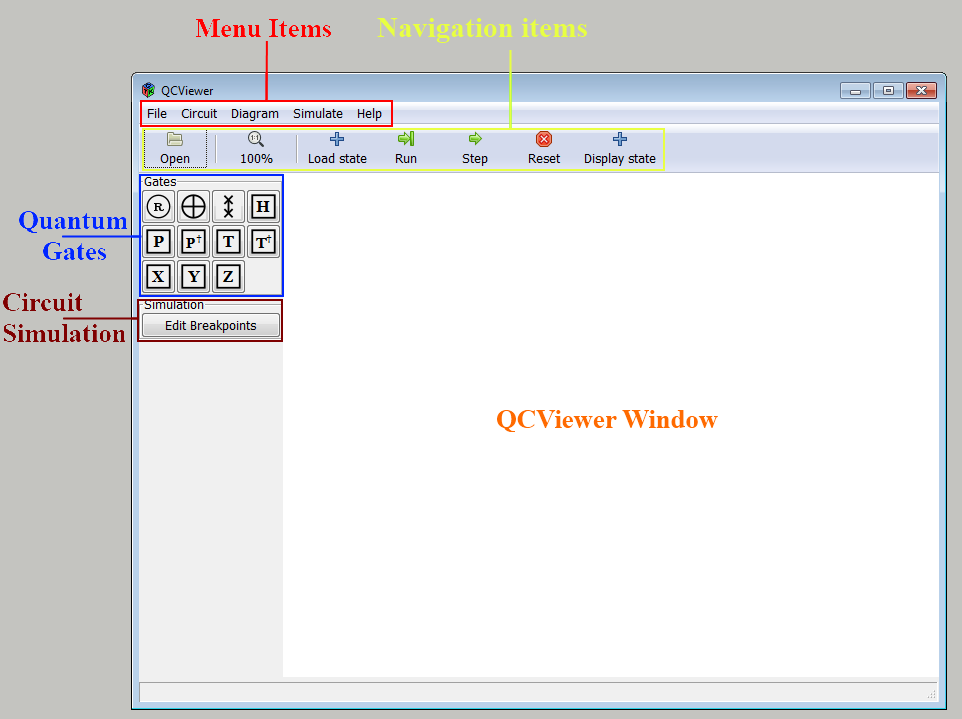
\includegraphics{figures/QCViewerGUI.png}
           \end{block}

           % Motivation Section
           \begin{block}{\large Motivation}
             In creating \textcolor{blue}{QCViewer}, our goal was to develop a convenient tool that would be useful to 
             the quantum computing community for both research and educational purposes. 
	\newline
	\\
             QCViewer provides a drag and drop interface for circuit design. This makes it easy to quickly 
             test out new algorithm and circuit design ideas. In order to make the diagrams useful for presentation 
             (e.g., Adobe Illustrator, PowerPoint) and publication (e.g., LaTex) we provide the ability to export 
             images in scalabe vector graphics (.svg) and portable network graphics (.png).

             \centering 
             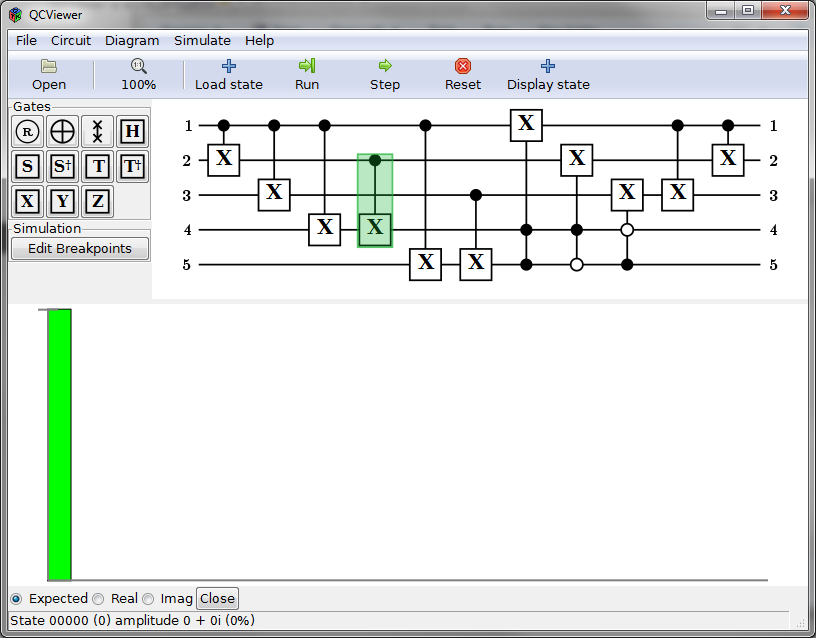
\includegraphics{figures/Motivation.png}
           \end{block}

         \end{minipage}
      \end{beamercolorbox}
    \end{column}

   % Circuit Design Section    
   \begin{column}{.33\textwidth}
      \begin{beamercolorbox}[center,wd=\textwidth]{postercolumn}
         \begin{minipage}[T]{.95\textwidth}
           \begin{block}{\large Circuit Design}
             Circuits can be designed on screen with drag and drop or by writing a ".qc" circuit file. Users have the choice of specifying circuits by either writing ASCII files directly or drawing them graphically. 

             \centering 
		\begin{figure}[!htbp]
		  \centering
		  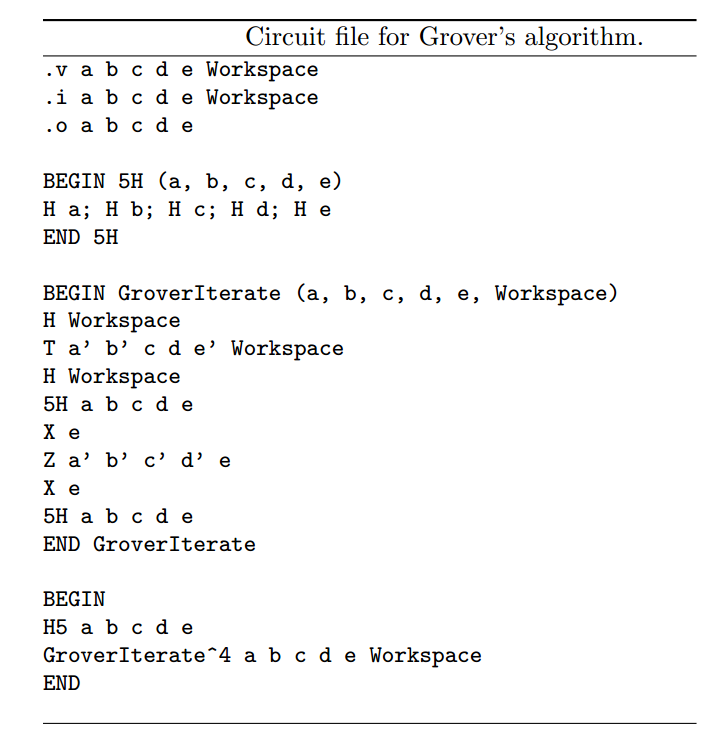
\includegraphics[height=3in]{figures/Grover_Text.PNG} \ \ \ \  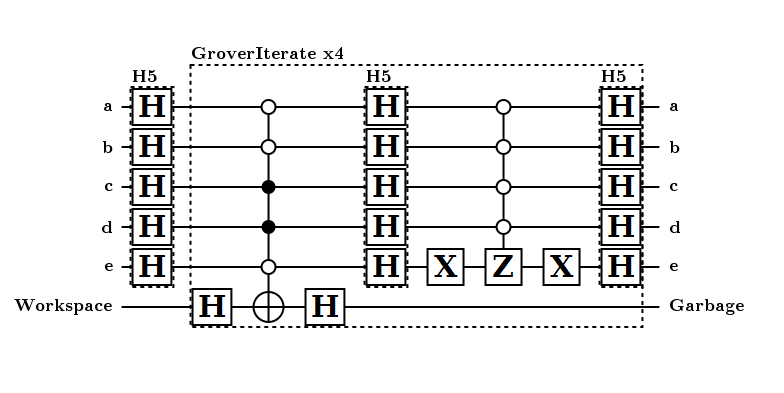
\includegraphics[height=3in]{figures/Grover_Circuit.PNG}
		  \caption{The ".qc" file format along with the corresponding graphical representation of Grover's circuit in QCViewer.}
		\end{figure}

The text on the left corresponds to a .qc specification of the corresponding circuit on the right. Circuit inputs and outputs are specified by the header information. The user may create a circuit block by beginning and ending with the "BEGIN" and "END" tags respectively. In between these tags, the circuit layout specifications are given as

\begin{align*}
\text{GATE \ GATE-WIRE \ CONTROLS[X] }
\end{align*}

where GATE is the name of some unitary gate, GATE-WIRE is the label relating to the wire on which the circuit is placed, and the CONTROLS[X]* are some finite list of possibly empty controlled operations corresponding to the gate.

             \centering 
		\begin{figure}[!htbp]
		  \centering
		  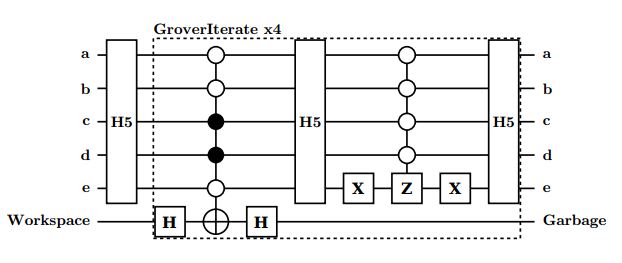
\includegraphics[height=3in]{figures/Grover_Loop.PNG} \ \ \ \ 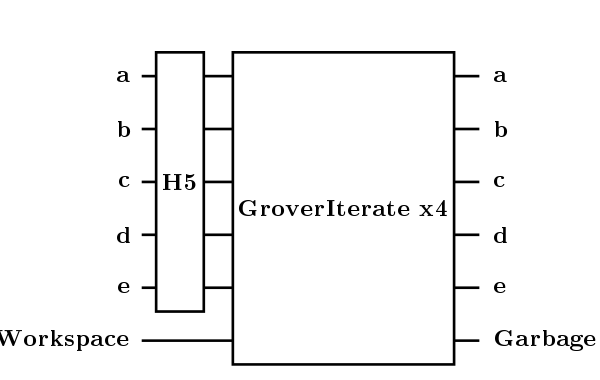
\includegraphics[height=3in]{figures/Grover_Roll.PNG} 
		  \caption{On the right, portions of Grover's circuit have been encapsulated in sub-circuit labels corresponding to specific portions of the circuit. The left image has the portions exposed and expanded.}
		\end{figure}

	    Filler words

             \centering 
		\begin{figure}[!htbp]
		  \centering
		  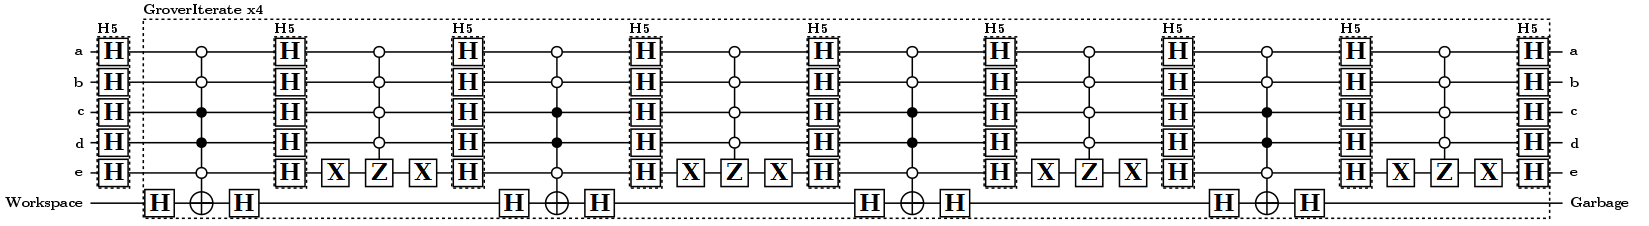
\includegraphics[width=14in]{figures/Grover_Unroll.PNG}
		  \caption{The above circuit of Grovers with the iteration and sub-circuits unrolled.}
		\end{figure}

           \end{block}

           % References Section
           \begin{block}{\large References}
		\begin{thebibliography}{9}
\small{
		\bibitem{Kliuchnikov12}
  		V. Kliuchnikov, D. Maslov, and M. Mosca,
  		\emph{Fast and Efficient Exact Synthesis of Single Qubit Unitaries Generated by Clifford T Gates}.
  		arXiv:1206.5236,
  		2012.

		\bibitem{Amy12}
  		M. Amy, D. Maslov, M. Mosca and M. Roetteler,
  		\emph{A Meet-in-the-Middle Algorithm for Fast Synthesis of Depth-Optimal Quantum Circuits}.
  		arXiv:1206.0758
  		2012.

		\bibitem{Maslov12}
  		D. Maslov,
  		\emph{Reversible Logic Synthesis Benchmarks Page}.
  		\href{http://webhome.cs.uvic.ca/~dmaslov/}{http://webhome.cs.uvic.ca/~dmaslov/}
  		2011.

		\bibitem{NC00}
  		M.A. Nielsen and I. L. Chuang, 
  		\emph{Quantum Computation and Quantum Information}.
  		Cambridge University Press,
		Cambridge New York,
  		2000.
}
		\end{thebibliography}
           \end{block}

         \end{minipage}
      \end{beamercolorbox}
    \end{column}

    % Circuit Simulation Section
    \begin{column}{.33\textwidth}
      \begin{beamercolorbox}[center,wd=\textwidth]{postercolumn}
         \begin{minipage}[T]{.95\textwidth}
           \begin{block}{\large Circuit Simulation}
              Our circuit simulator is state-vector based.

                    \centering 
		\begin{figure}[!htbp]
		  \centering
		  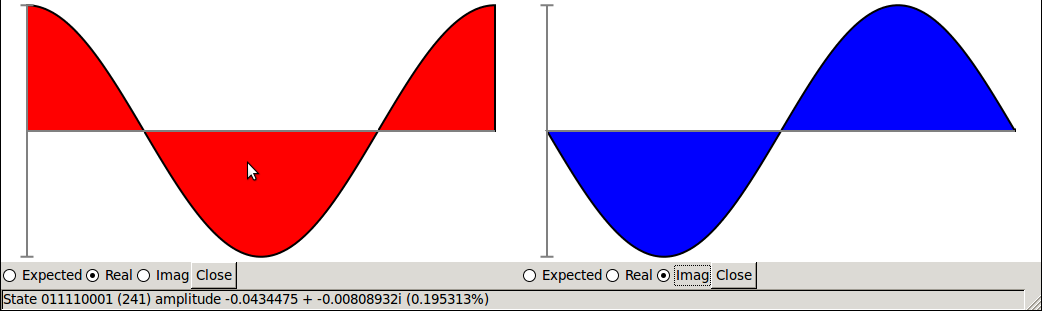
\includegraphics{figures/state.PNG}
		  \caption{Grover circuit and corresponding text.}
		\end{figure}

	         Filler

                    \centering 
		\begin{figure}[!htbp]
		  \centering
		  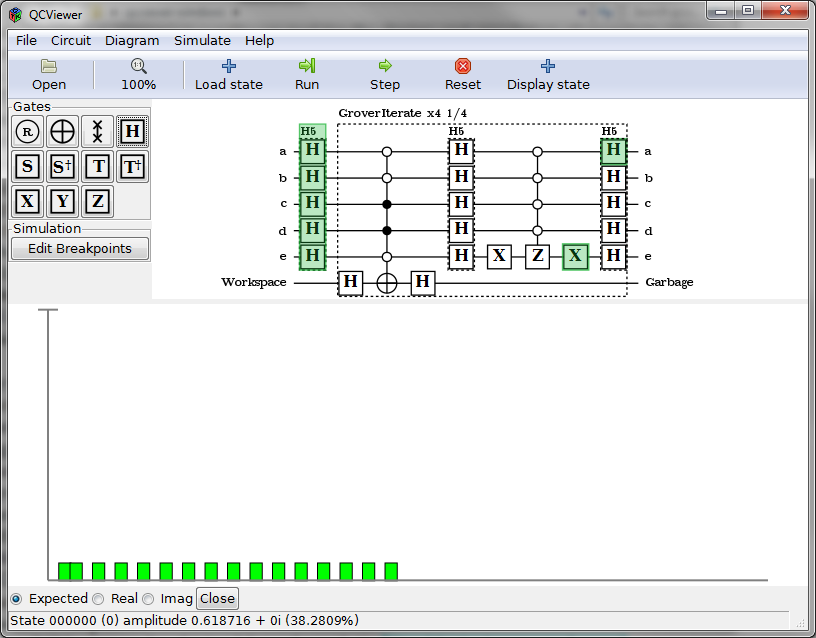
\includegraphics[width=7in]{figures/Grover_Simulate1.PNG} \ \  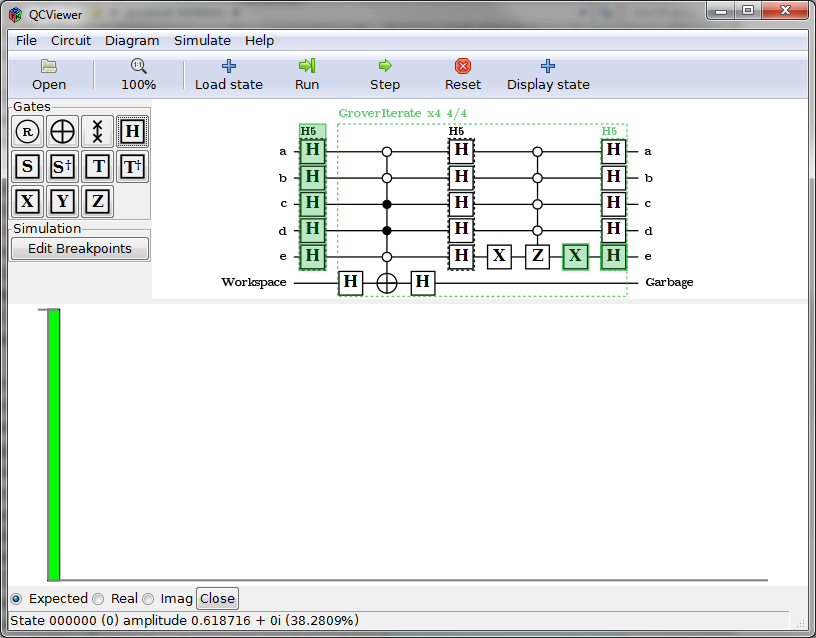
\includegraphics[width=7in]{figures/Grover_Simulate2.PNG}
		  \caption{Grover circuit and corresponding text.}
		\end{figure}

           \end{block}

           % Acknowledgments Section
           \begin{block}{\large Acknowledgments}
             \centering 
             
\includegraphics[height=1in]{figures/CIFAR_Logo.PNG} \ \ 
\includegraphics[height=1in]{figures/IQC_Logo.PNG}  \ \ 
\includegraphics[height=1in]{figures/NSERC_Logo.PNG}

            This work has been supported in part by the Institute for Quantum Computing and the Perimeter Institute for Theoretical Physics. We also thank NSERC, CIFAR, QuantumWorks, and the University of Waterloo.

             \centering 
             
\includegraphics[height=2in]{figures/Waterloo_Logo.PNG} \ \ 
\includegraphics[height=2in]{figures/PI_Logo.PNG} \ \ 
\includegraphics[height=2in]{figures/QuantumWorks_Logo.PNG}
           \end{block}

         \end{minipage}
      \end{beamercolorbox}
    \end{column}




  \end{columns}
  \end{frame}
\end{document}
